% ================================================================
\chapter{Árvores geradoras mínimas: Kruskal e Prim}\label{cap:agm}\label{sec:agm}
% ================================================================
\begin{objetivos}
\begin{itemize}
  \item O problema da árvore geradora mínima e a propriedade do corte.
  \item O algoritmo de Kruskal, com Union-Find, e a sua correção.
  \item O algoritmo de Prim e as suas implementações com vetor, heap binário e heap de Fibonacci.
  \item Como escolher a implementação de acordo com a densidade do grafo.
\end{itemize}
\end{objetivos}

Ligar $n$ cidades por uma rede de custo mínimo, usando apenas as ligações possíveis, é encontrar uma \textbf{árvore geradora mínima} (AGM). Os dois algoritmos clássicos são gulosos: o de Kruskal percorre as arestas em ordem crescente de peso e aceita as que não fecham ciclo, usando a estrutura Union-Find do Capítulo~\ref{cap:uf}; o de Prim faz crescer uma única árvore a partir de uma raiz, usando uma fila de prioridades (Capítulos~\ref{cap:heap} e~\ref{cap:heapav}). A correção dos dois decorre de um único lema, a propriedade do corte.

\section{O problema e a propriedade do corte}
Dado um grafo conexo $G$ com pesos $c$ nas arestas, queremos uma \textbf{árvore geradora} --- um subgrafo conexo e acíclico que contém todos os $n$ vértices e, portanto, tem $n-1$ arestas --- de peso total mínimo. Um \textbf{corte} $(S,V\setminus S)$ é uma partição dos vértices em dois lados, e uma aresta \textbf{atravessa} o corte se tem um extremo em cada lado.
\begin{lema}[Propriedade do corte]\label{lema:corte}
Seja $A$ um conjunto de arestas contido em alguma AGM e $(S,V\setminus S)$ um corte que nenhuma aresta de $A$ atravessa. Se $e$ é uma aresta de peso mínimo entre as que atravessam o corte, então $A\cup\{e\}$ está contido em alguma AGM.
\end{lema}
\begin{proof}
Seja $T$ uma AGM com $A\subseteq T$. Se $e\in T$, não há o que provar. Senão, $T+e$ tem um ciclo que passa por $e$; como $e$ atravessa o corte, o ciclo precisa atravessá-lo de novo, por outra aresta $f\in T$, e $f\notin A$, pois nenhuma aresta de $A$ atravessa o corte. Então $T'=T+e-f$ é uma árvore geradora e $c(T')=c(T)+c(e)-c(f)\le c(T)$, pois $c(e)\le c(f)$. Logo $T'$ é uma AGM e contém $A\cup\{e\}$.
\end{proof}

\section{O algoritmo de Kruskal}\label{sec:kruskal}
No algoritmo de Kruskal, a solução parcial é uma \textbf{floresta}. As arestas são percorridas em ordem crescente de peso, e cada uma é aceita se \textbf{não forma ciclo} com as já aceitas, isto é, se liga duas árvores diferentes da floresta. O teste é feito com conjuntos disjuntos: cada árvore da floresta é um conjunto, e uma aresta $uv$ fecha ciclo se e somente se $u$ e $v$ estão no mesmo conjunto.
\begin{pseudo}{Kruskal com Union-Find}
\begin{algorithmic}
\Function{Kruskal}{$G,c$}
  \State $E(T):=\emptyset$
  \For{\textbf{cada} $v\in V$} \State \MakeSet$(v)$ \Comment{$n$ árvores com um vértice} \EndFor
  \State ordene as arestas de modo que $c(e_1)\le c(e_2)\le\dots\le c(e_m)$ \Comment{$O(m\log m)=O(m\log n)$}
  \For{$j:=1$ \textbf{até} $m$}
    \State seja $e_j=uv$
    \If{\Find$(u)\ne$ \Find$(v)$} \Comment{une duas árvores distintas: não fecha ciclo}
      \State $E(T):=E(T)\cup\{e_j\}$;\ \Union$(u,v)$
    \EndIf
  \EndFor
  \State \Return $T$ \Comment{pode parar quando $|E(T)|=n-1$}
\EndFunction
\end{algorithmic}
\end{pseudo}
\textbf{Complexidade.} A ordenação domina: $O(m\log m)=O(m\log n)$, pois $m\le n^2$ implica $\log m\le2\log n$. O laço custa $O(m+n\log n)$ com listas encadeadas e união ``menor na maior'', já que cada vértice muda de conjunto no máximo $\log n$ vezes, ou $O(m\,\alpha(n))$ com floresta, rank e compressão de caminhos. O total é $O(m\log n)$.

\textbf{Correção.} Ao aceitar $e=uv$, tome como $S$ a árvore atual de $u$. Nenhuma aresta aceita atravessa esse corte, e $e$ é a mais leve que o atravessa: uma aresta mais leve que o atravessasse teria sido examinada antes, quando os seus extremos já estavam em árvores diferentes (as árvores só crescem), e teria sido aceita. Pelo Lema~\ref{lema:corte}, por indução, o conjunto de arestas aceitas está sempre contido numa AGM. O algoritmo de Kruskal também é o Teorema~\ref{teo:gulosomat} aplicado à matroide gráfica.

\begin{center}
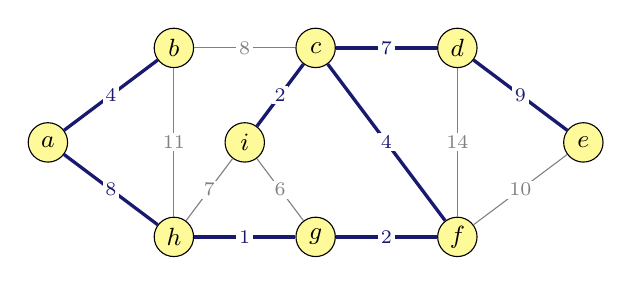
\begin{tikzpicture}[v/.style={circle,draw,fill=yellow!40,inner sep=1.2pt,minimum size=5mm,font=\small},
  agm/.style={very thick,MidnightBlue}, nao/.style={thin,gray}, w/.style={font=\scriptsize,fill=white,inner sep=1pt}]
\node[v] (a) at (0,1.2) {$a$}; \node[v] (b) at (1.6,2.4) {$b$}; \node[v] (c) at (3.4,2.4) {$c$}; \node[v] (d) at (5.2,2.4) {$d$};
\node[v] (e) at (6.8,1.2) {$e$}; \node[v] (f) at (5.2,0) {$f$}; \node[v] (g) at (3.4,0) {$g$}; \node[v] (h) at (1.6,0) {$h$};
\node[v] (i) at (2.5,1.2) {$i$};
\draw[agm] (a)--node[w]{4}(b); \draw[agm] (a)--node[w]{8}(h); \draw[nao] (b)--node[w]{11}(h); \draw[nao] (b)--node[w]{8}(c);
\draw[nao] (h)--node[w]{7}(i); \draw[agm] (h)--node[w]{1}(g); \draw[agm] (i)--node[w]{2}(c); \draw[nao] (i)--node[w]{6}(g);
\draw[agm] (c)--node[w]{7}(d); \draw[agm] (c)--node[w]{4}(f); \draw[agm] (g)--node[w]{2}(f); \draw[nao] (d)--node[w]{14}(f);
\draw[agm] (d)--node[w]{9}(e); \draw[nao] (e)--node[w]{10}(f);
\end{tikzpicture}
\end{center}
\begin{exemplo}[Kruskal e Prim no grafo acima]\label{ex:agm}
O algoritmo de Kruskal aceita $hg\,(1)$, $ic\,(2)$, $gf\,(2)$, $ab\,(4)$, $cf\,(4)$, $cd\,(7)$, $ah\,(8)$ e $de\,(9)$, e rejeita $ig\,(6)$, $hi\,(7)$, $bc\,(8)$, $ef\,(10)$, $bh\,(11)$ e $df\,(14)$, que fechariam ciclos. A AGM tem \textbf{custo 37} (arestas em azul). O algoritmo de Prim, com raiz $a$, acrescenta $ab\,(4)$, $ah\,(8)$, $hg\,(1)$, $gf\,(2)$, $fc\,(4)$, $ci\,(2)$, $cd\,(7)$ e $de\,(9)$, nessa ordem, e chega à mesma árvore. A AGM não é única: $ah$ e $bc$ pesam 8, e trocar uma pela outra dá outra AGM de custo 37. Quando todos os pesos são distintos, a AGM é única.
\end{exemplo}

\section{O algoritmo de Prim}\label{sec:prim}
No algoritmo de Prim, a solução parcial é uma \textbf{árvore} que cresce a partir de uma raiz: a cada passo, entra a aresta mais leve com um extremo na árvore e o outro fora dela. A correção vem do Lema~\ref{lema:corte}, com $S=V(T)$.
\begin{pseudo}{Prim em $O(n^2)$ com vetores}
\begin{algorithmic}
\Function{Prim}{$G,W,r$}
  \State para todo $v$: $chave(v):=\infty$;\ $pai(v):=\nil$;\ $dentro(v):=$ falso
  \State $chave(r):=0$
  \For{$it:=1$ \textbf{até} $n$}
    \State $u:=$ vértice com $dentro(u)=$ falso e $chave(u)$ mínima \Comment{varredura em $O(n)$}
    \State $dentro(u):=$ verdadeiro \Comment{se $u\ne r$, a aresta $pai(u)\,u$ entra na árvore}
    \For{\textbf{cada} $v\in N(u)$ com $dentro(v)=$ falso} \Comment{matriz: linha $u$, $O(n)$; listas: $O(\text{grau}(u))$}
      \If{$W(u,v)<chave(v)$} \State $chave(v):=W(u,v)$;\ $pai(v):=u$ \EndIf
    \EndFor
  \EndFor
  \State \Return $\{\,pai(v)\,v : v\ne r\,\}$
\EndFunction
\end{algorithmic}
\end{pseudo}
O valor $chave(v)$ é o peso da aresta mais leve que liga $v$ à árvore. O algoritmo tem o mesmo esqueleto do algoritmo de Dijkstra (Capítulo~\ref{cap:dijkstra}), trocando ``$L(u)+W(u,v)$'' por ``$W(u,v)$''.
\begin{center}\small
\begin{tabularx}{\linewidth}{@{}>{\raggedright\arraybackslash}p{5.2cm}>{\raggedright\arraybackslash}p{3.6cm}X@{}}
\toprule
Implementação & Custo & Comentário\\
\midrule
Matriz de adjacência e vetor $chave$ & $O(n^2)$ & $n$ varreduras de $O(n)$; ótimo para matriz\\
Listas de adjacência e vetor $chave$ & $O(n^2+m)=O(n^2)$ & a varredura domina\\
Listas e heap binário (com redução de chave) & $O(m\log n)$ & $n$ remoções e até $m$ reduções, cada uma $O(\log n)$\\
Listas e heap de Fibonacci & $O(m+n\log n)$ & redução de chave em $O(1)$\am\\
\bottomrule
\end{tabularx}
\end{center}
A versão com heap \textbf{não é necessariamente melhor} que a de $O(n^2)$: num grafo denso, $m=\Theta(n^2)$ e $m\log n=\Theta(n^2\log n)$. O heap compensa quando $m=o(n^2/\log n)$.

\begin{cuidado}[Armadilhas de árvores geradoras mínimas]
\begin{itemize}
  \item ``O guloso funciona porque escolhe o melhor a cada passo'' não é uma prova. A prova é a propriedade do corte, ou a estrutura de matroide.
  \item O algoritmo de Kruskal aceita uma aresta se ela \emph{não fecha ciclo}, e não ``se o vértice ainda não foi visitado'' --- isso seria o algoritmo de Prim. No Kruskal, a solução parcial pode ser desconexa.
  \item A AGM minimiza a soma dos pesos, e não as distâncias até uma raiz; isso é o que faz o algoritmo de Dijkstra.
  \item A complexidade do Kruskal é $O(m\log n)$ por causa da \emph{ordenação}; as operações de Union-Find, sozinhas, são quase lineares.
  \item O Prim com heap não é sempre melhor; em grafos densos, perde para a versão com vetor.
\end{itemize}
\end{cuidado}

\begin{chave}
Propriedade do corte: a aresta mais leve que atravessa um corte que $A$ não atravessa pode ser acrescentada a $A$. Kruskal: arestas em ordem crescente e Union-Find, $O(m\log n)$. Prim: uma árvore que cresce pela aresta mais leve do corte, $O(n^2)$ com vetor ou matriz, $O(m\log n)$ com heap binário ou $O(m+n\log n)$ com heap de Fibonacci. Com pesos distintos, a AGM é única.
\end{chave}

% ----------------------------------------------------------------
\section{Exercícios}
\excurso
\begin{exercicio}{agm-l1}[Lista]
Prove a correção do algoritmo de Kruskal.
\end{exercicio}
\begin{exercicio}{agm-l2}[Lista]
Prove a correção do algoritmo de Prim.
\end{exercicio}
\begin{exercicio}{agm-l3}[Lista]
Mostre como implementar o algoritmo de Prim em tempo $O(m\log n)$ com o grafo representado por listas de adjacência.
\end{exercicio}
\begin{exercicio}{agm-l4}[Lista]
Mostre como implementar o algoritmo de Prim em tempo $O(n^2)$ com o grafo representado (a) por listas de adjacência; (b) por matriz de adjacência.
\end{exercicio}
\begin{exercicio}{agm-l6}[Lista]
É possível implementar o algoritmo de Prim em tempo $O(n^2)$ com matriz de adjacência? É possível fazer melhor que isso nessa representação? Justifique.
\end{exercicio}
\begin{exercicio}{agm-l7}[Lista]
Quais seriam as formas de resolver o problema da árvore geradora de peso \textbf{máximo}? Justifique.
\end{exercicio}

\excompl
\begin{exercicio}{agm-sim}[Complementar]
No grafo com as arestas $AB\,(6)$, $AC\,(1)$, $AD\,(5)$, $BC\,(5)$, $BE\,(3)$, $CD\,(5)$, $CE\,(6)$, $CF\,(4)$, $DF\,(2)$ e $EF\,(6)$, execute o Kruskal (indicando as arestas rejeitadas) e o Prim a partir de $A$ (indicando a ordem de entrada das arestas). Qual o custo da AGM? Ela é única?
\end{exercicio}
\begin{exercicio}{agm-unica}[Complementar]
Prove que, se todos os pesos são distintos, a AGM é única.
\end{exercicio}
\begin{exercicio}{agm-ciclo}[Complementar]
Prove a \emph{propriedade do ciclo}: se $e$ é a aresta de peso estritamente maior de algum ciclo de $G$, então $e$ não pertence a nenhuma AGM.
\end{exercicio}
\begin{exercicio}{agm-gargalo}[Complementar]
Mostre que, numa AGM $T$, o caminho entre dois vértices $u$ e $v$ minimiza o peso da \emph{maior} aresta, entre todos os caminhos de $u$ a $v$ em $G$.
\end{exercicio}
\begin{exercicio}{agm-nova}[Complementar]
Dada uma AGM $T$ de $G$, acrescenta-se a $G$ uma nova aresta $uv$ de peso $c$. Como obter uma AGM do novo grafo em $O(n)$?
\end{exercicio}
\begin{exercicio}{agm-prim7}[Complementar]
No grafo com as arestas $AB\,(7)$, $AD\,(5)$, $BC\,(8)$, $BD\,(9)$, $BE\,(7)$, $CE\,(5)$, $DE\,(15)$, $DF\,(6)$, $EF\,(8)$, $EG\,(9)$ e $FG\,(11)$, execute o Prim a partir de $A$, mostrando a ordem em que as arestas entram, e o Kruskal, mostrando as arestas rejeitadas. Qual o custo da AGM?
\end{exercicio}
\begin{exercicio}{agm-boruvka}[Complementar \estrela]
No algoritmo de Borůvka, cada componente da floresta atual escolhe, em paralelo, a aresta mais leve que sai dela, e todas essas arestas são acrescentadas de uma vez. Mostre que o algoritmo está correto (supondo pesos distintos) e que faz $O(\log n)$ rodadas, cada uma em $O(m)$.
\end{exercicio}
\begin{exercicio}{agm-iguais}[Complementar]
Se todas as arestas têm o mesmo peso, como encontrar uma AGM em $O(n+m)$?
\end{exercicio}
\begin{exercicio}{agm-12}[Complementar]
Se todos os pesos são 1 ou 2, mostre como encontrar uma AGM em $O(m\,\alpha(n))$, sem ordenar por comparações.
\end{exercicio}
\begin{exercicio}{agm-leve}[Complementar]
Prove que, se a aresta mais leve do grafo é única, ela pertence a toda AGM. Vale o mesmo para a segunda mais leve? E para a terceira?
\end{exercicio}
\begin{exercicio}{agm-dijk}[Complementar]
Dê um grafo conexo com pesos positivos em que a árvore de caminhos mínimos a partir de algum vértice (Capítulo~\ref{cap:dijkstra}) não é uma AGM.
\end{exercicio}
\begin{exercicio}{agm-parar}[Complementar]
No algoritmo de Kruskal, quantas arestas são examinadas no melhor e no pior caso, se o laço para ao aceitar $n-1$ arestas? Isso muda a complexidade assintótica?
\end{exercicio}
\begin{exercicio}{agm-listas}[Complementar]
Explique por que, no algoritmo de Kruskal com Union-Find por listas encadeadas e união ``menor na maior'', o laço principal custa $O(m+n\log n)$.
\end{exercicio}
\begin{exercicio}{agm-floresta}[Complementar]
Se o grafo é desconexo, o que o algoritmo de Kruskal devolve? E o de Prim? Como obter uma \emph{floresta geradora mínima}?
\end{exercicio}
\begin{exercicio}{agm-segunda}[Complementar \estrela]
A \emph{segunda melhor} árvore geradora é a de menor peso entre as diferentes de uma AGM fixada $T$. Mostre que ela pode ser obtida de $T$ trocando uma única aresta, e dê um algoritmo $O(n^2)$ para encontrá-la.
\end{exercicio}
